\section{基于Zigzag映射矩阵的时间隐通道评估}
\label{chap:zigzag:results}
本节对基于Zigzag的时间隐通道进行评估,参照时间隐通道的构造指标,评估由抗检测能力、鲁棒性、传输性能及构建代价四个方面组成。其中,抗检测能力测试按照本文\nref{chap:analyze:statistical}提出的检测方法进行。

\subsection{评估环境及参数}
\label{chap:zigzag:results:environment}
该时间隐通道构建方法中,主要的参数为$L_{Codeword}$,其取值决定了传输性能,并对抗检测能力有显著影响。实验的测试场景,为本文\nref{chap:analyze:results}中表\nref{tab:3:capture-results}两种场景下的测试数据,以及随机生成的网络噪声。

\insertTable{
	\begin{table}[htbp]
      \centering
      \caption{测试环境信息表}
      \label{tab:4:result:environment}
          \begin{tabular*}{0.9\textwidth}{@{\extracolsep{\fill}}cc}
            \toprule
            类型 & 详细信息 \\
            \midrule
            PC平台 & I5-9400,DDR4 16GB \\
            软件版本 & Windows 7,QT 5.9.5,python 3.6;Ubuntu 16.04,mysql 5.7 \\
            数据集 & VoLTE抓包结果,随机噪声 \\
            \bottomrule
          \end{tabular*}
    \end{table}
}

评估实验的软硬件环境如表\nref{tab:4:result:environment},所有的数据均存储到mysql数据库中,通过基于QT的时间隐通道处理逻辑,得到调制与解调结果。根据调制解调结果,评估抗检测能力等指标。基于python脚本,将抓包结果还原为视频数据,并评估调制前后的视频质量,得到隐通道构建代价测试结果。此外,为有效评估鲁棒性、比较不同丢包率下的误码率水平,随机生成了丢包率为0.5\%、1\%、2\%、5\%、10\%的五种噪声。

\insertTable{
	\begin{table}[htbp]
      \centering
      \caption{基于Zigzag映射矩阵时间隐通道的参数}
      \label{tab:4:parameters}
          \begin{tabular*}{0.5\textwidth}{@{\extracolsep{\fill}}ccc}
            \toprule
            $L_{Codeword}$\ (bits) & $2^{L_{Codeword}}$ & 主动丢包率 \\
            \midrule
            7 & 128 & 0.781\% \\ 
            8 & 256 & 0.391\% \\ 
            9 & 512 & 0.195\% \\ 
            10 & 1024 & 0.098\% \\ 
            11 & 2048 & 0.049\% \\ 
            \bottomrule
          \end{tabular*}
    \end{table}
}

参照本文\nref{chap:analyze:result}的实验结果,设定参数$L_{Codeword}$取值如表\nref{tab:4:parameters},在能够通过检测的前提下进行其他测试。

\subsection{抗检测能力测试}
\label{chap:zigzag:results:undetectability}

按照本文\nref{chap:analyze:statistical}中提出的时间隐通道检测方法,对基于Zigzag映射矩阵的时间隐通道进行抗检测能力评估,评估方式及参数保持一致。

\subsubsection{IPD检测}
\label{chap:zigzag:results:undetectability:ipd}

\insertFigure{
	\begin{figure}[htbp]
        \centering
        \subfigure[Excellent场景的CDF]{
            \label{fig:4:results:ipd:cdf:excellent}
            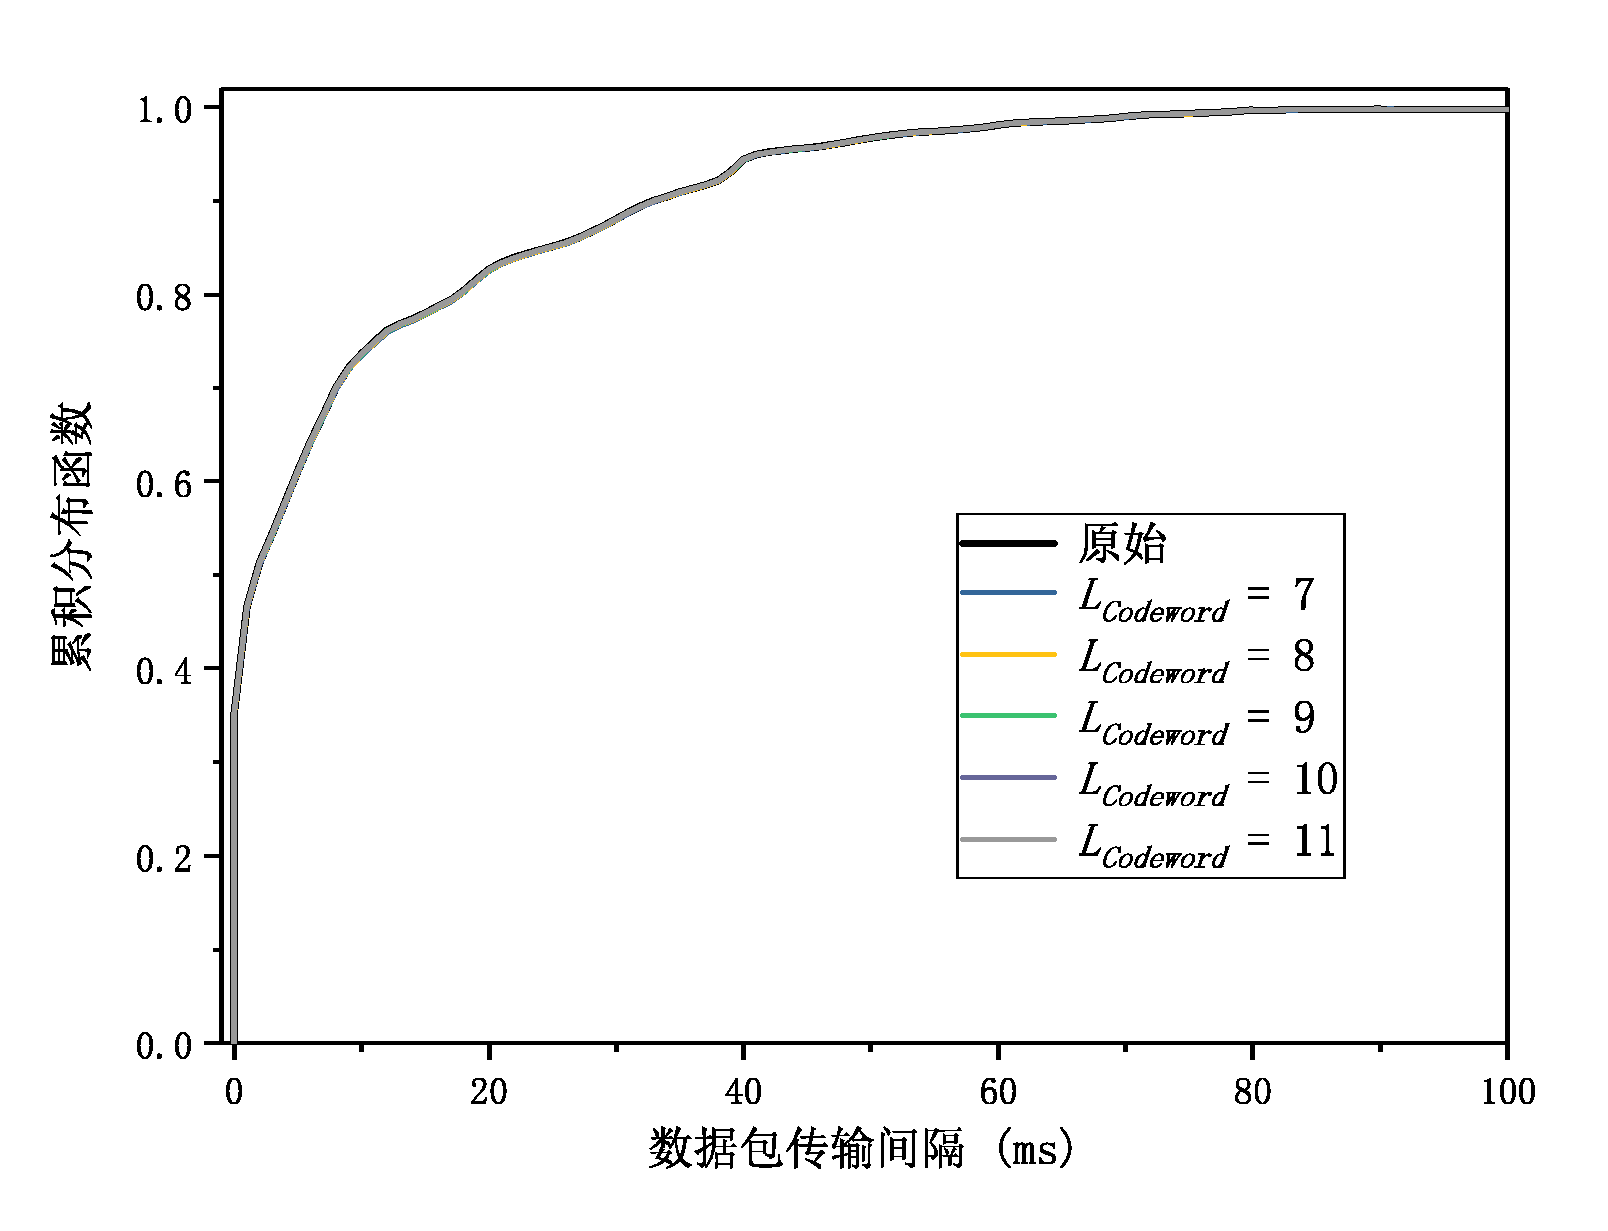
\includegraphics[width=0.48\textwidth]{chapters/chapter4/figures/ipd-cdf-excellent.pdf}
        }
        \subfigure[Good场景的CDF]{
            \label{fig:4:results:ipd:cdf:good}
            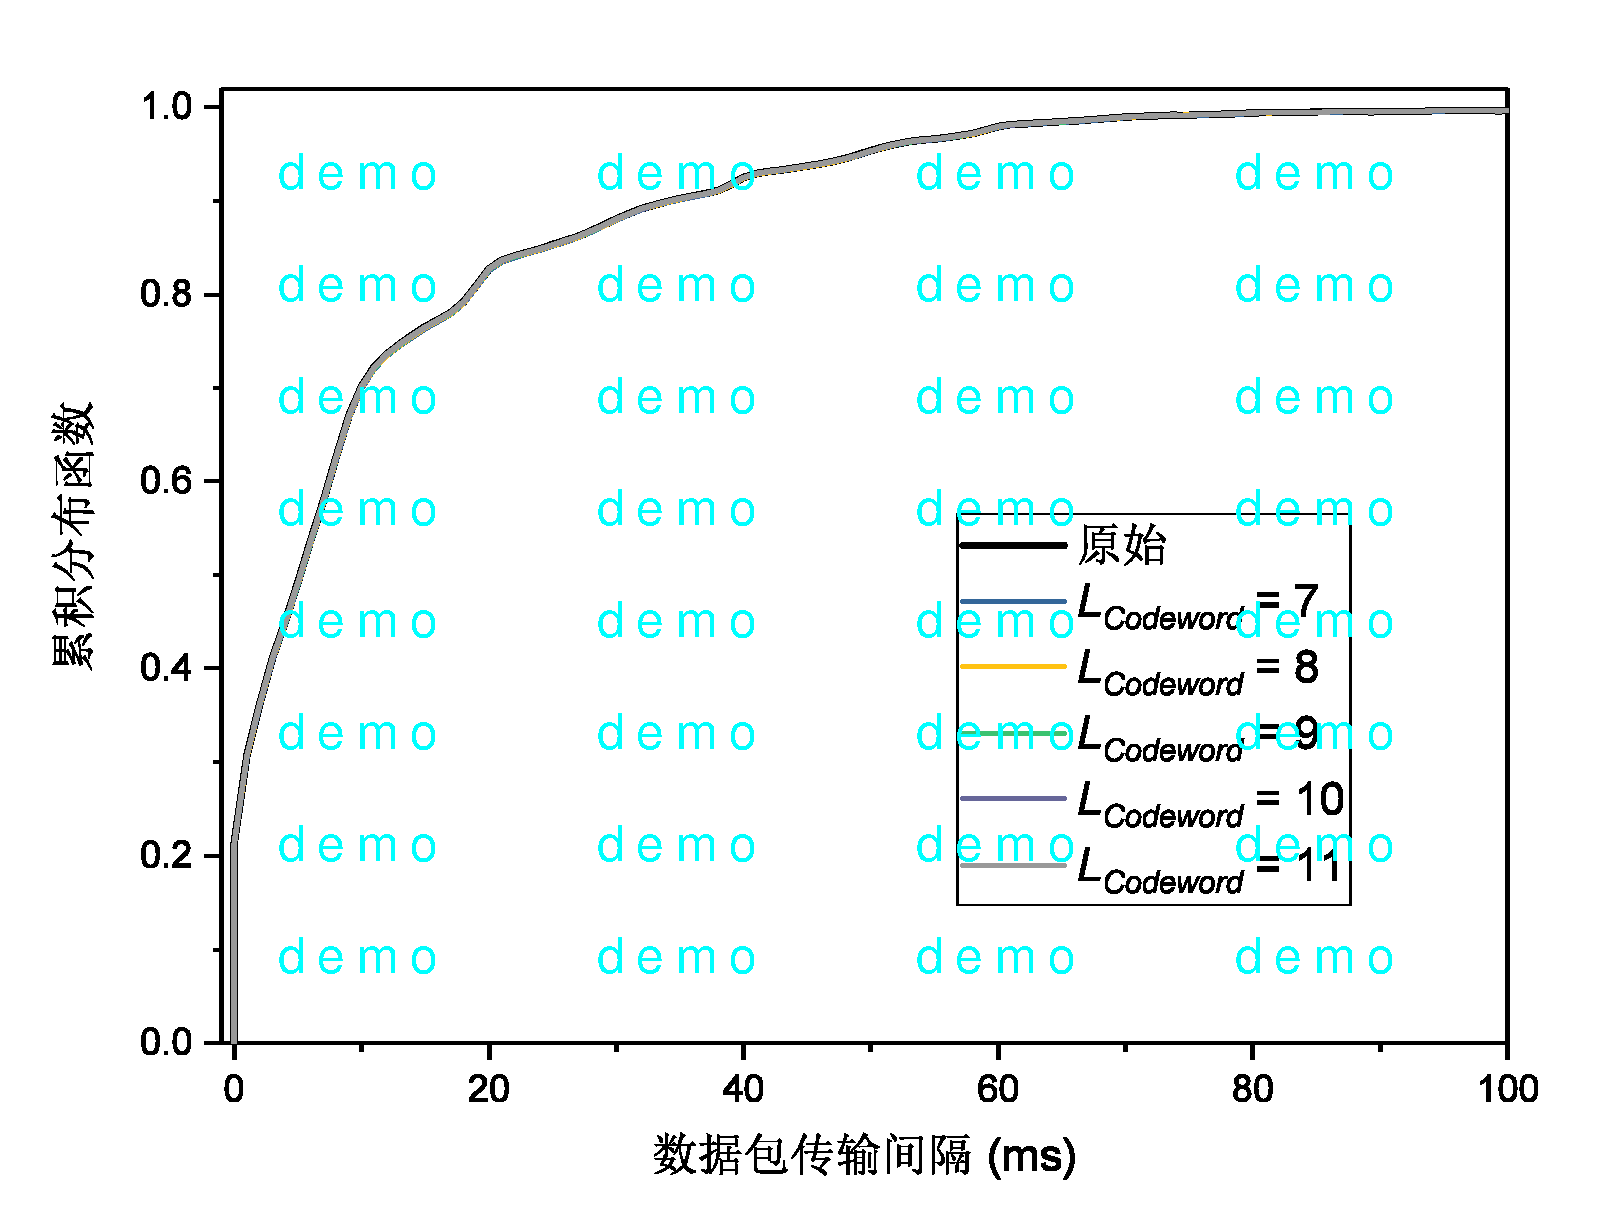
\includegraphics[width=0.48\textwidth]{chapters/chapter4/figures/ipd-cdf-good.pdf}
        }
        \caption{IPD分布的CDF曲线}
        \label{fig:4:results:ipd:cdf}
    \end{figure}
}

\insertTable{
	\begin{table}[htbp]
        \centering
        \caption{IPD检测检出率汇总表}
        \label{tab:4:results:ipd}
        \begin{threeparttable}
            \begin{tabular*}{0.85\textwidth}{@{\extracolsep{\fill}}ccc}
                \toprule
                $L_{Codeword}$ & 方法 & 检出率\\ 
                \midrule
                \multirow{5}{*}{7,8,9,10,11} 
                & K-S检验 & 0\% \\
                & Welch's t检验, Mann–Whitney rank检验\tnote{1} & 0\% \\
                & K-L散度 & 0\% \\
                & Wasserstein距离 & 0\% \\
                & 能量距离 & 0\% \\
                \bottomrule
            \end{tabular*}
            \begin{tablenotes}
                \footnotesize
                \item[1] Welch's t检验与Mann–Whitney rank检验通过一种即可
            \end{tablenotes}
        \end{threeparttable}
    \end{table}
}

IPD分布的CDF曲线如图\nref{fig:4:results:ipd:cdf}所示,在两种不同的场景中,通过IPD的CDF曲线已经无法区分该时间隐通道。该结果与本文\nref{chap:analyze:result:ipd:cdf}中的测试结果统一,当$L_{Codeword}\ge 7$时,在IPD分布上已经没有显著的差异,基于IPD的检测方法无法检测出该时间隐通道。

IPD的量化检测结果如表\nref{tab:4:results:ipd},设定的参数在所有的场景中,该时间隐通道均无法被检测出来。检测结果证明,该时间隐通道在IPD分布方面抗检测能力,满足时间隐通道的隐蔽性要求。

\subsubsection{突发丢包长度检测}
\label{chap:zigzag:results:undetectability:burst}

\insertFigure{
    \begin{figure}[htbp]
        \centering
        \subfigure[Excellent场景的CDF]{
            \label{fig:4:results:burst:cdf:excellent}
            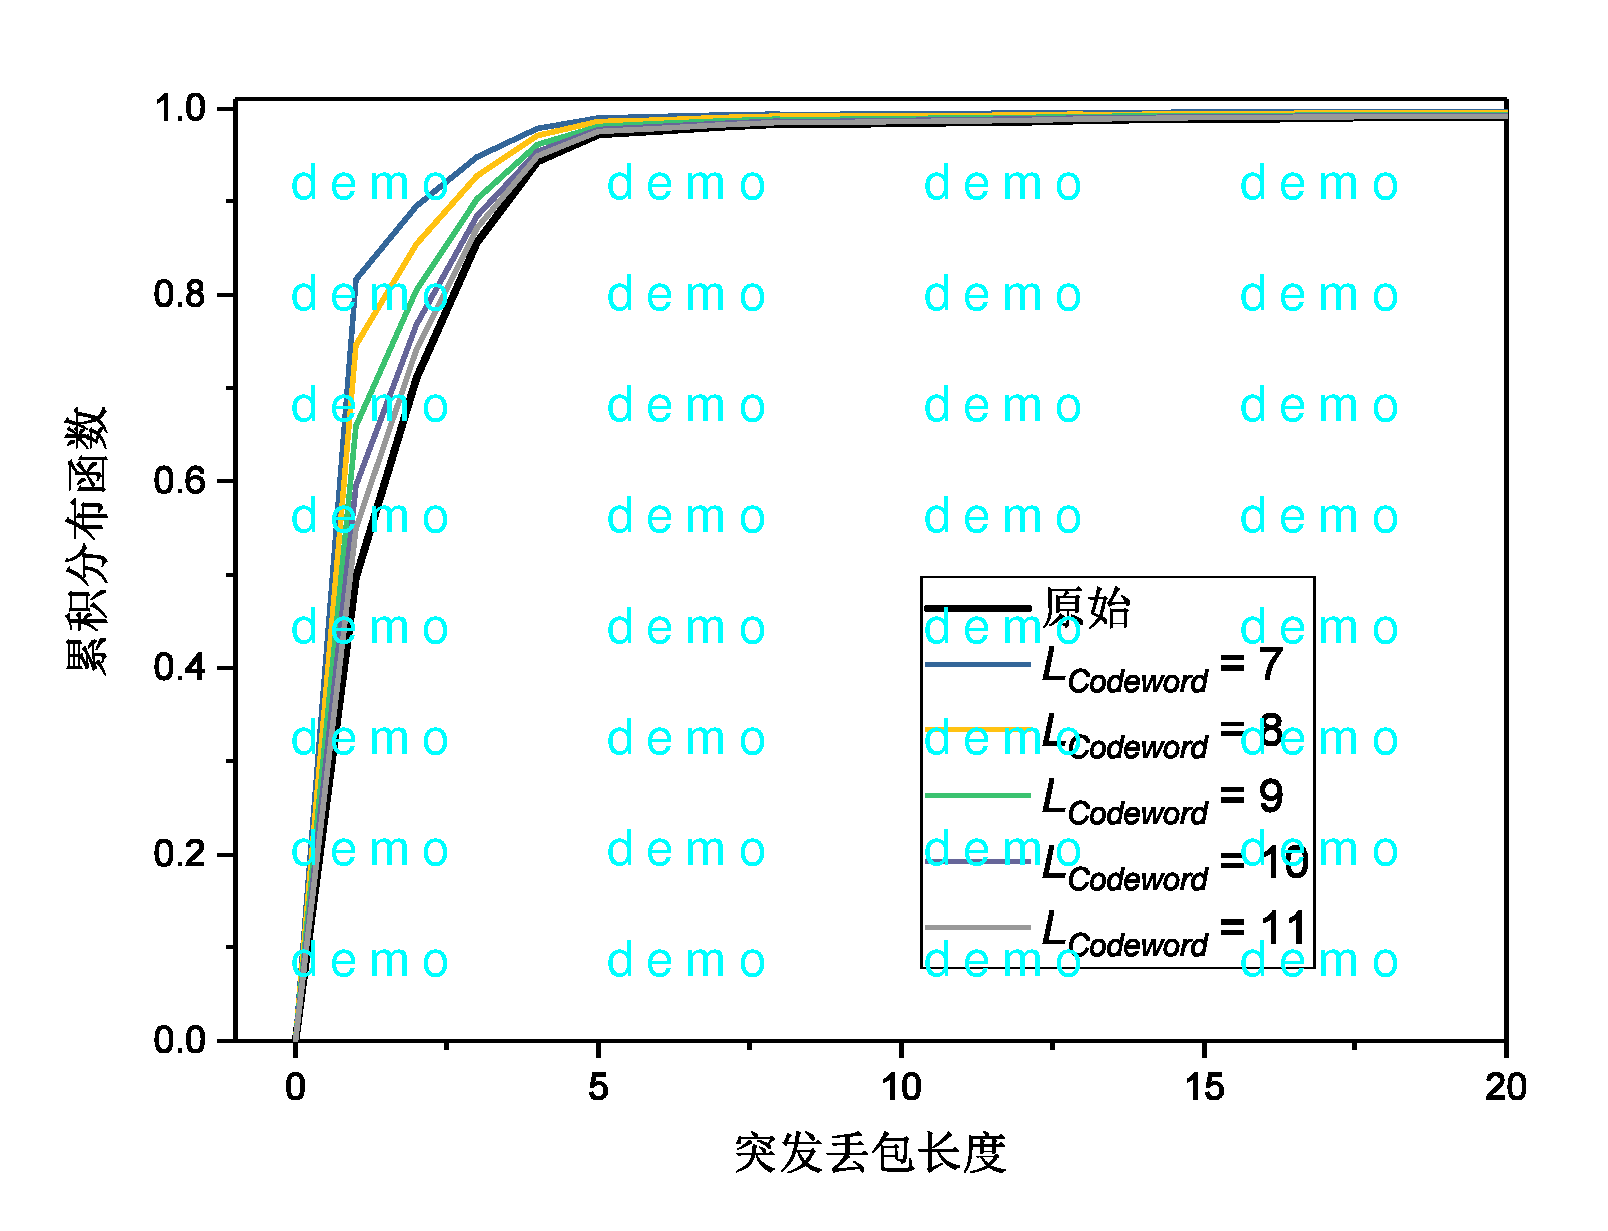
\includegraphics[width=0.48\textwidth]{chapters/chapter4/figures/burst-cdf-excellent.pdf}
        }
        \subfigure[Good场景的CDF]{
            \label{fig:4:results:burst:cdf:good}
            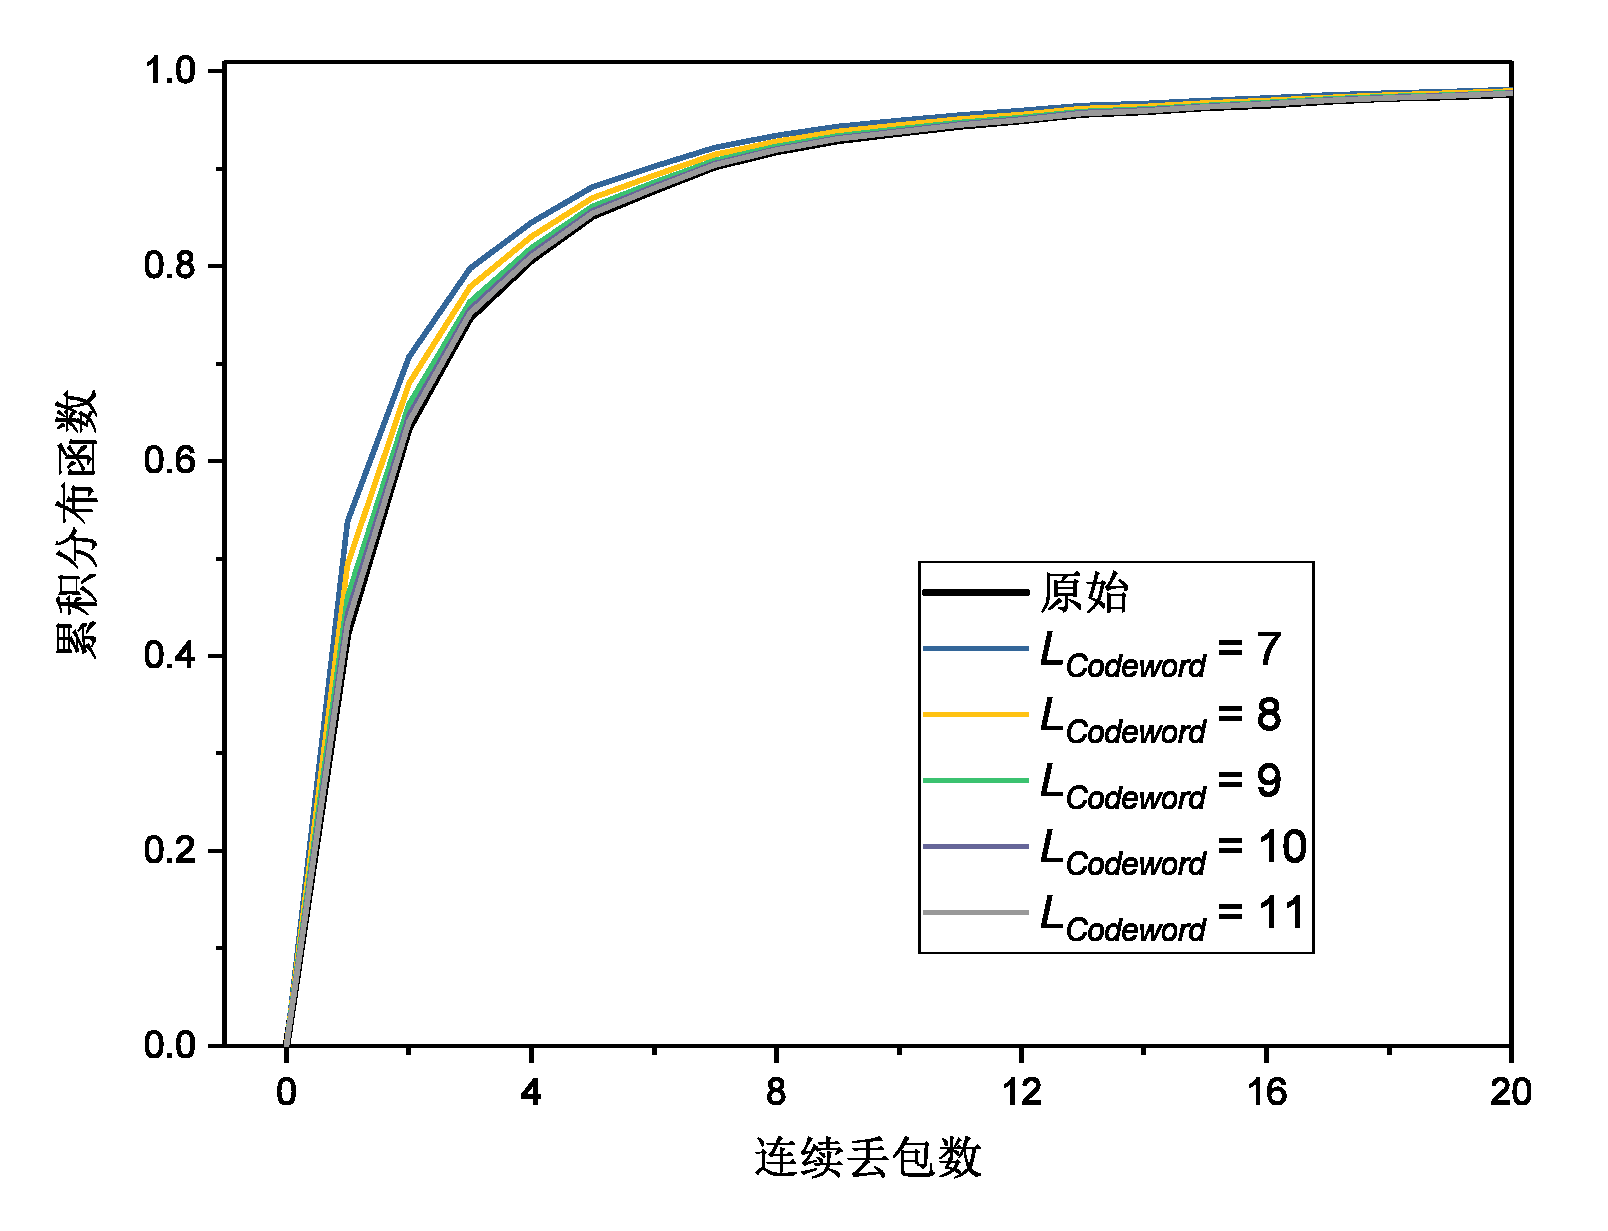
\includegraphics[width=0.48\textwidth]{chapters/chapter4/figures/burst-cdf-good.pdf}
        }
        \caption{突发丢包长度的CDF曲线}
        \label{fig:4:results:burst:cdf}
    \end{figure}
}

\insertTable{
	\begin{table}[htbp]
      \centering
      \caption{突发丢包长度检测检出率汇总表}
      \label{tab:4:results:burst}
          \begin{tabular*}{0.75\textwidth}{@{\extracolsep{\fill}}cccc}
            \toprule
            场景 & $L_{Codeword}$ & 方法 & 检出率 \\ 
            \midrule
            \multirow{4}{*}{Excellent} 
            & 7,8 & K-L散度 & 100\% \\
            & 9,10,11 & K-L散度 & 0\% \\
            & 7,8,9,10,11 & Wasserstein距离 & 0\% \\
            & 7,8,9,10,11 & 能量距离 & 0\% \\
            \\
            \multirow{3}{*}{Good}
            & 7,8,9,10,11 & K-L散度 & 0\% \\
            & 7,8,9,10,11 & Wasserstein距离 & 0\% \\
            & 7,8,9,10,11 & 能量距离 & 0\% \\
            \bottomrule
          \end{tabular*}
    \end{table}
}

突发丢包长度的CDF,如图\nref{fig:4:results:burst:cdf}。两种场景中,时间隐通道的曲线均出现了一定偏离,并且Excellent场景中的差异更加明显。总体来说,随着$L_{Codeword}$的增大,时间隐通道的分布与原始分布更加接近,与理论预期一致。参照表\nref{tab:4:parameters},参数$L_{Codeword}$与主动丢包率呈负相关,减少丢包则减弱对分布的影响。

突发丢包长度检测的量化评估结果,如表\nref{tab:4:results:burst}。Excellent场景中,当$L_{Codeword}\ge 9$时,已经无法检测出时间隐通道;而Good场景中,设定参数下已经无法检测出时间隐通道。因此,要通过突发丢包长度检测,Excellent场景下$L_{Codeword}$至少为9,Good场景下$L_{Codeword}\ge 7$即可满足要求。

\subsubsection{区间丢包数检测}
\label{chap:zigzag:results:undetectability:win}

\insertFigure{
    \begin{figure}[htbp]
        \centering
        \subfigure[窗口100时Excellent场景的CDF]{
            \label{fig:4:results:win100:cdf:excellent}
            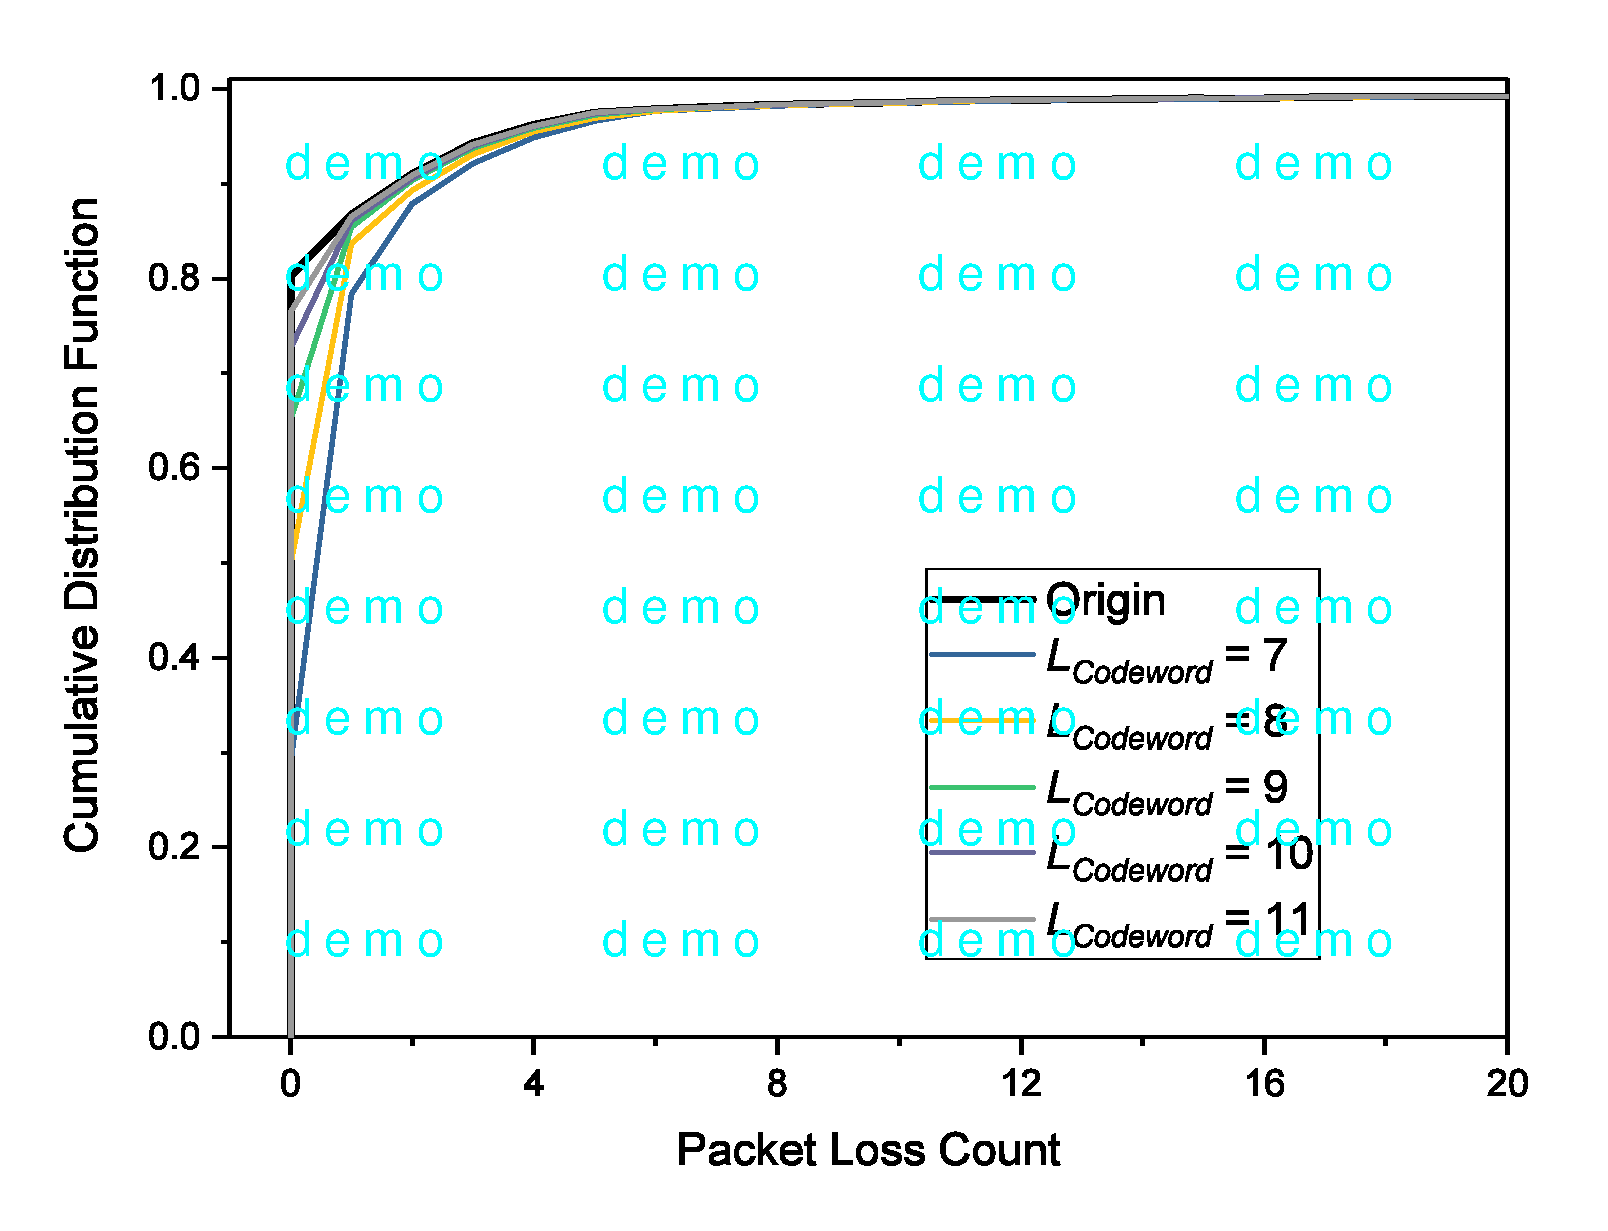
\includegraphics[width=0.48\textwidth]{chapters/chapter4/figures/win100-cdf-excellent.pdf}
        }
        \subfigure[窗口100时Good场景的CDF]{
            \label{fig:4:results:win100:cdf:good}
            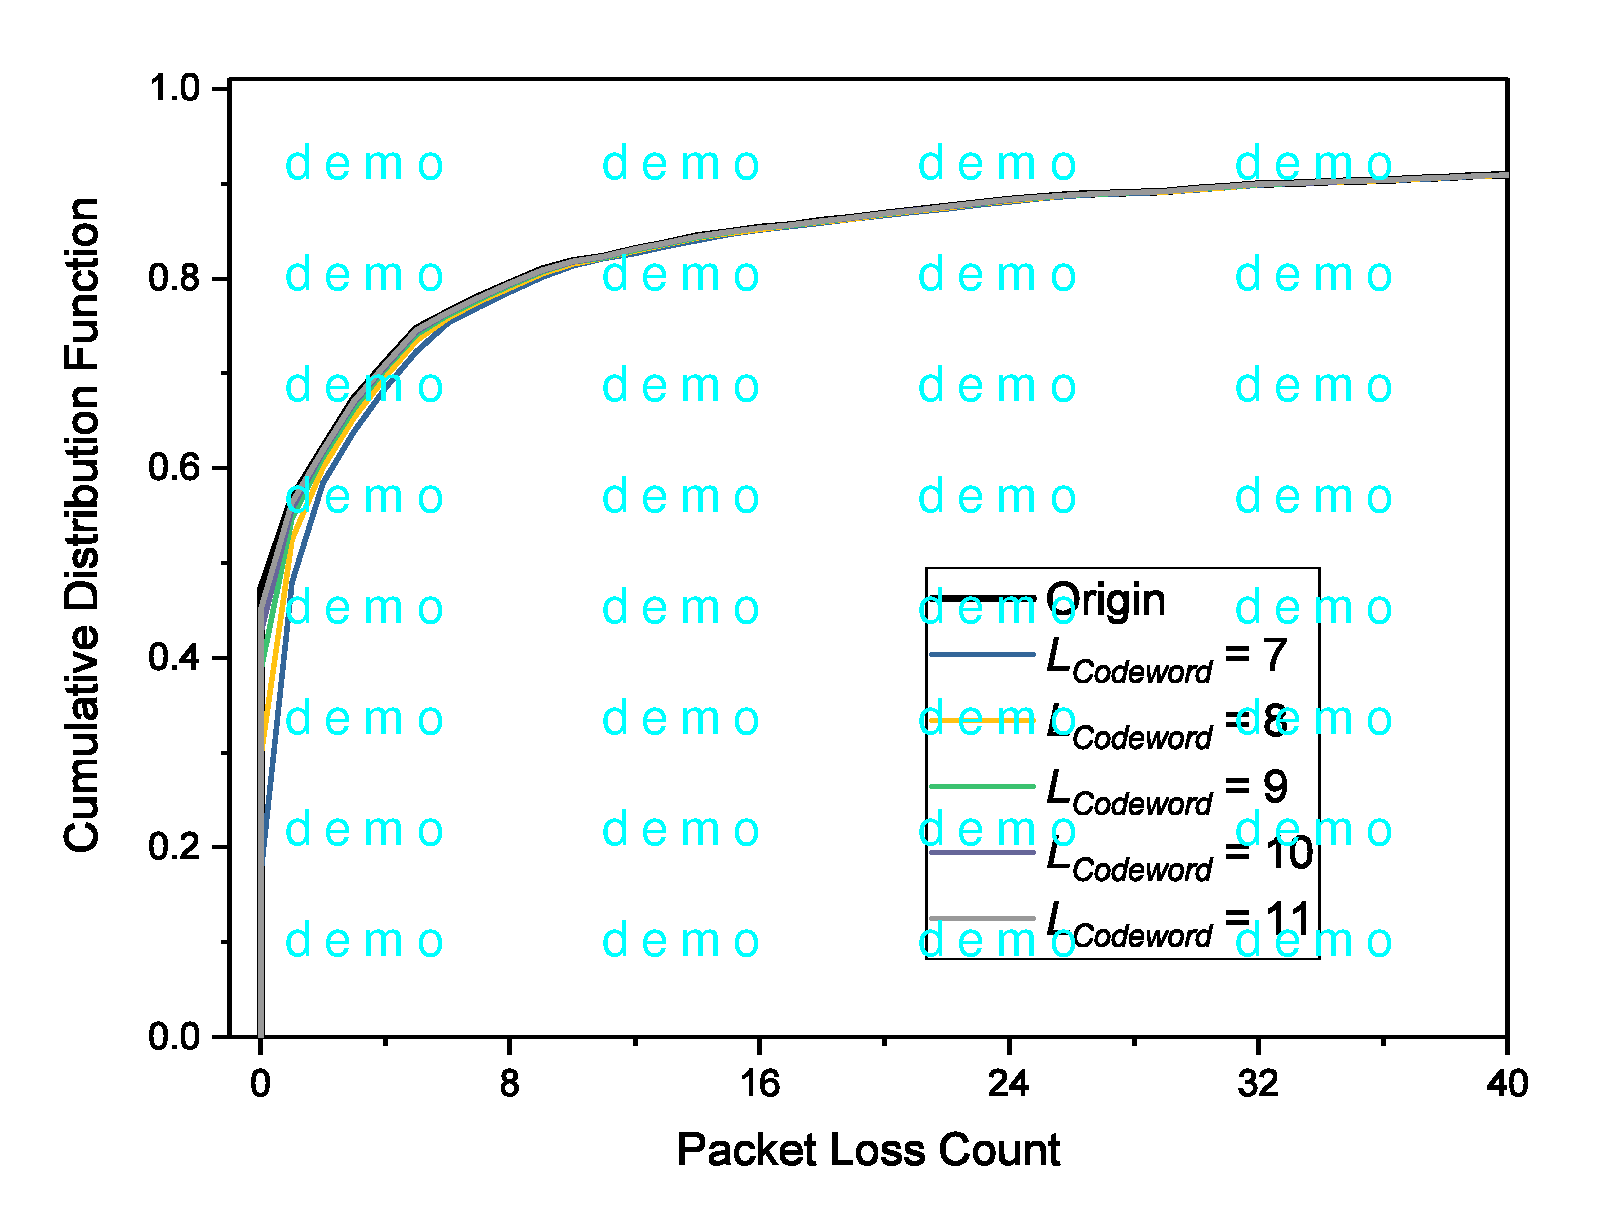
\includegraphics[width=0.48\textwidth]{chapters/chapter4/figures/win100-cdf-good.pdf}
        }
        \subfigure[窗口200时Excellent场景的CDF]{
            \label{fig:4:results:win200:cdf:excellent}
            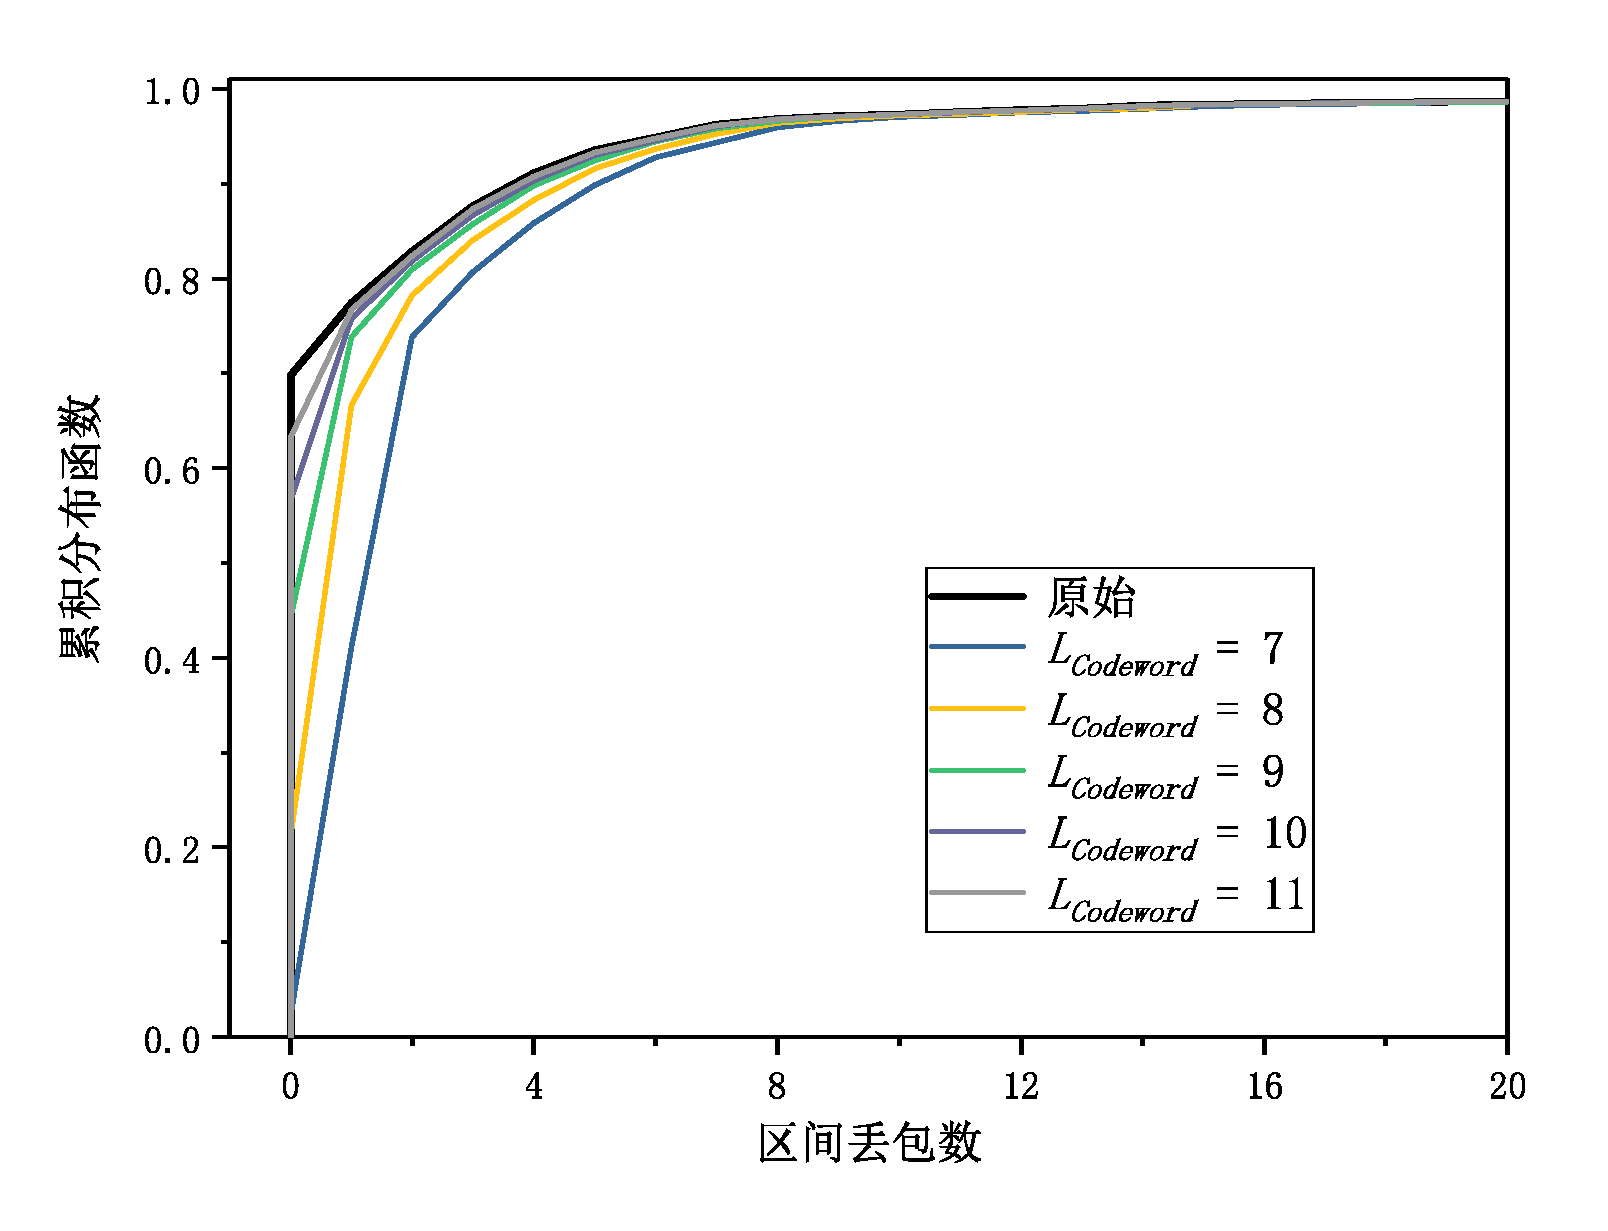
\includegraphics[width=0.48\textwidth]{chapters/chapter4/figures/win200-cdf-excellent.pdf}
        }
        \subfigure[窗口200时Good场景的CDF]{
            \label{fig:4:results:win200:cdf:good}
            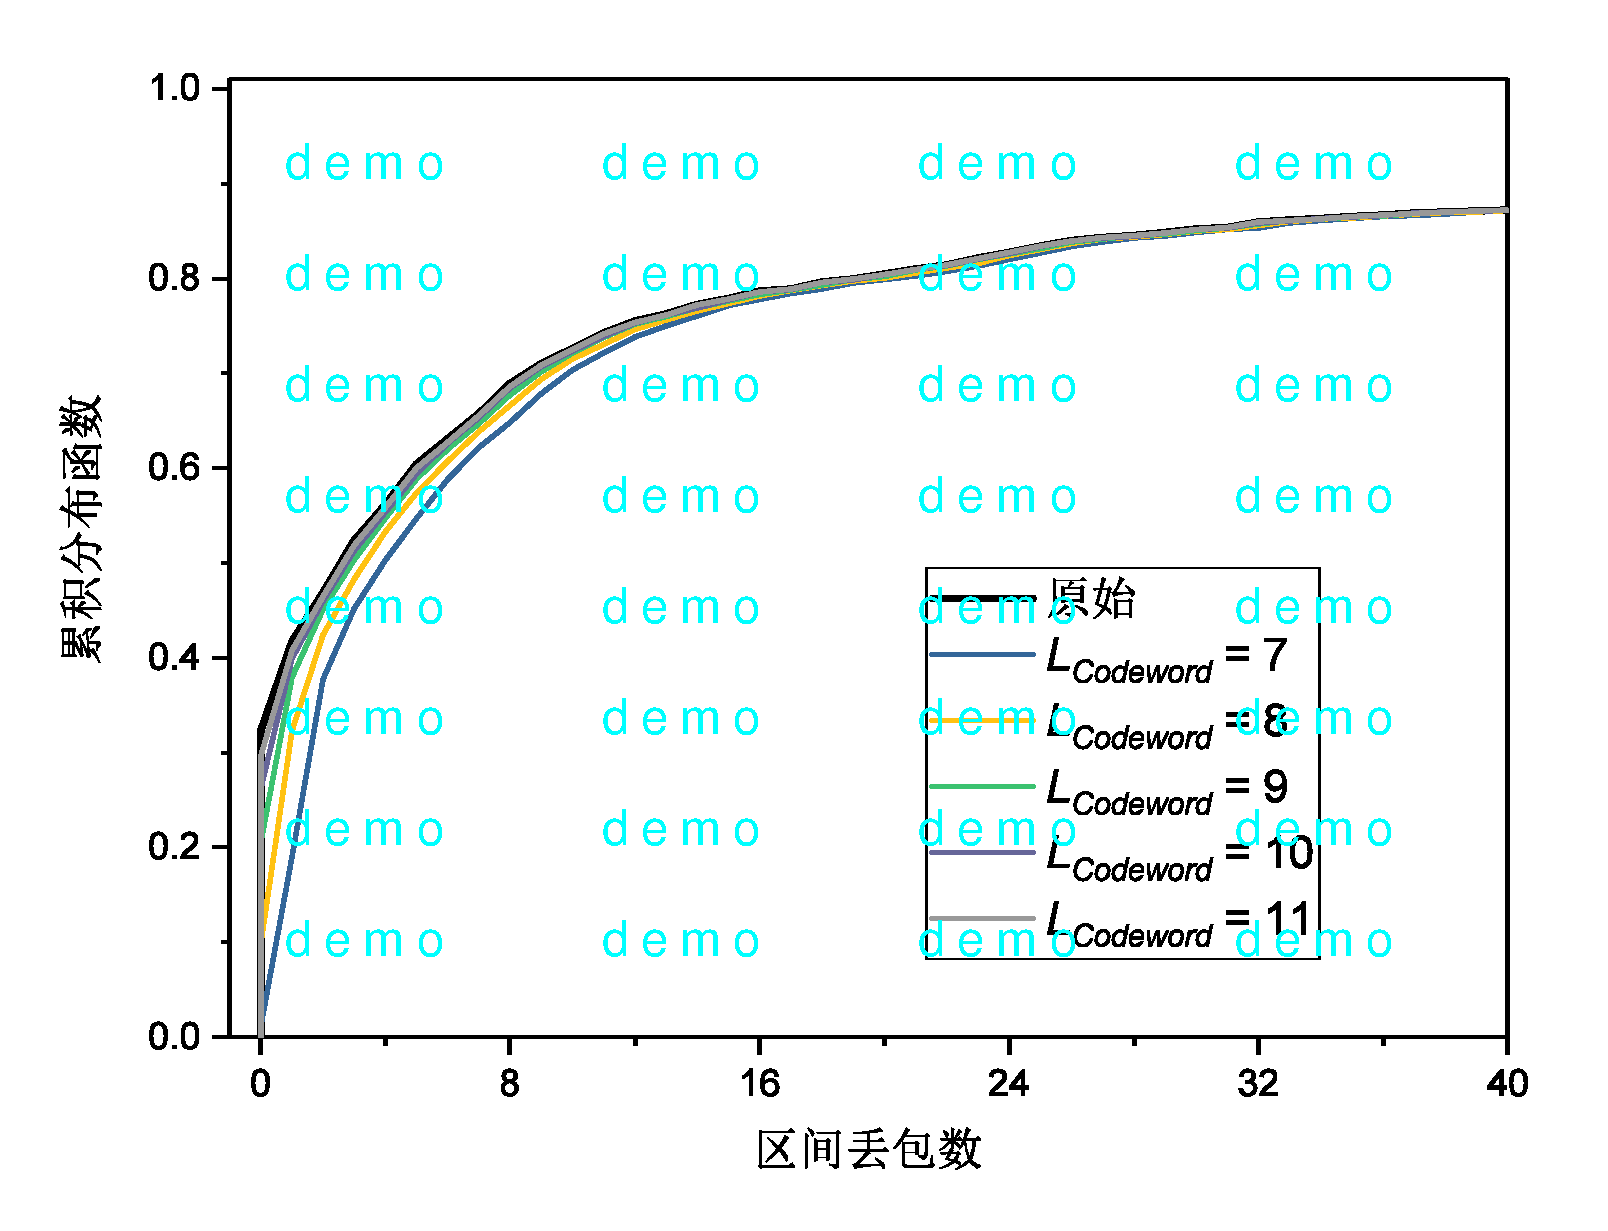
\includegraphics[width=0.48\textwidth]{chapters/chapter4/figures/win200-cdf-good.pdf}
        }
        \caption{区间丢包数的CDF曲线}
        \label{fig:4:results:win:cdf}
    \end{figure}
}

\insertTable{
	\begin{table}[htbp]
      \centering
      \caption{区间丢包数检测检出率汇总表}
      \label{tab:4:results:win}
          \begin{tabular*}{0.75\textwidth}{@{\extracolsep{\fill}}cccc}
            \toprule
            场景 & $L_{Codeword}$ & 方法 & 检出率 \\ 
            \midrule
            \multirow{4}{*}{Excellent} 
            & 7 & Wasserstein距离 & 100\% \\
            & 8,9,10,11 & Wasserstein距离 & 0\% \\
            & 7 & 能量距离 & 100\% \\
            & 8,9,10,11 & 能量距离 & 0\% \\
            \\
            \multirow{6}{*}{Good}
            & 7 & Wasserstein距离 & 100\% \\
            & 8 & Wasserstein距离 & 30\% \\
            & 9,10,11 & Wasserstein距离 & 0\% \\
            & 7 & 能量距离 & 100\% \\
            & 8 & 能量距离 & 30\% \\
            & 9,10,11 & 能量距离 & 0\% \\
            \bottomrule
          \end{tabular*}
    \end{table}
}

在区间丢包数检测中,窗口长度与本文\nref{chap:analyze:result:window}保持一致,分别为100及200。区间丢包数的CDF曲线如图\nref{fig:4:results:win:cdf},本时间隐通道CDF曲线的起始位置没有发生显著偏移,与本文\nref{chap:analyze:result:window}的检测结果基本一致。

区间丢包数检测的量化结果,如表\nref{tab:4:results:win},Wasserstein距离及能量距离具备良好检测能力。Excellent场景下,当$L_{Codeword}\ge 8$时即可通过检测;而Good场景下,当$L_{Codeword}\ge 9$时才可以通过所有检测。

\subsubsection{抗检测能力测试汇总}
\label{chap:zigzag:results:undetectability:all}

\insertTable{
	\begin{table}[htbp]
      \centering
      \caption{基于Zigzag映射矩阵的时间隐通道检出率汇总表}
      \label{tab:4:results:sum}
          \begin{tabular*}{0.8\textwidth}{@{\extracolsep{\fill}}cccccc}
            \toprule
            \multirow{2}{*}{场景} 
            & \multicolumn{5}{c}{$L_{Codeword}$} \\
            & 7 & 8 & 9 & 10 & 11 \\
            \midrule
            Excellent & 100\% & 100\% & 0\% & 0\% & 0\% \\
            Good & 100\% & 30\% & 0\% & 0\% & 0\% \\
            \bottomrule
          \end{tabular*}
    \end{table}
}

基于Zigzag映射矩阵的时间隐通道,其抗检测能力测试的最终结果如表\nref{tab:4:results:sum}。当$L_{Codeword}\ge 9$时,即可在所有场景中通过检测;当$L_{Codeword} = 8$时,在Good场景下有一定几率通过检测。通过对比发现,Excellent场景对主动丢包的容忍度有限,传输参数需要保守设定。

通过抗检测能力测试,本方法通过调整传输参数$L_{Codeword}$,在各种通话场景下均可通过测试。测试结果与表\nref{tab:3:result-sum:all}基本一致,同时验证了该方法及时间隐通道检测方法。

\subsection{鲁棒性测试}
\label{chap:zigzag:results:robustness}

\insertFigure{
	\begin{figure}[htbp]
        \centering
        \subfigure[Excellent及Good场景]{
            \label{fig:4:results:ber:scenario}
            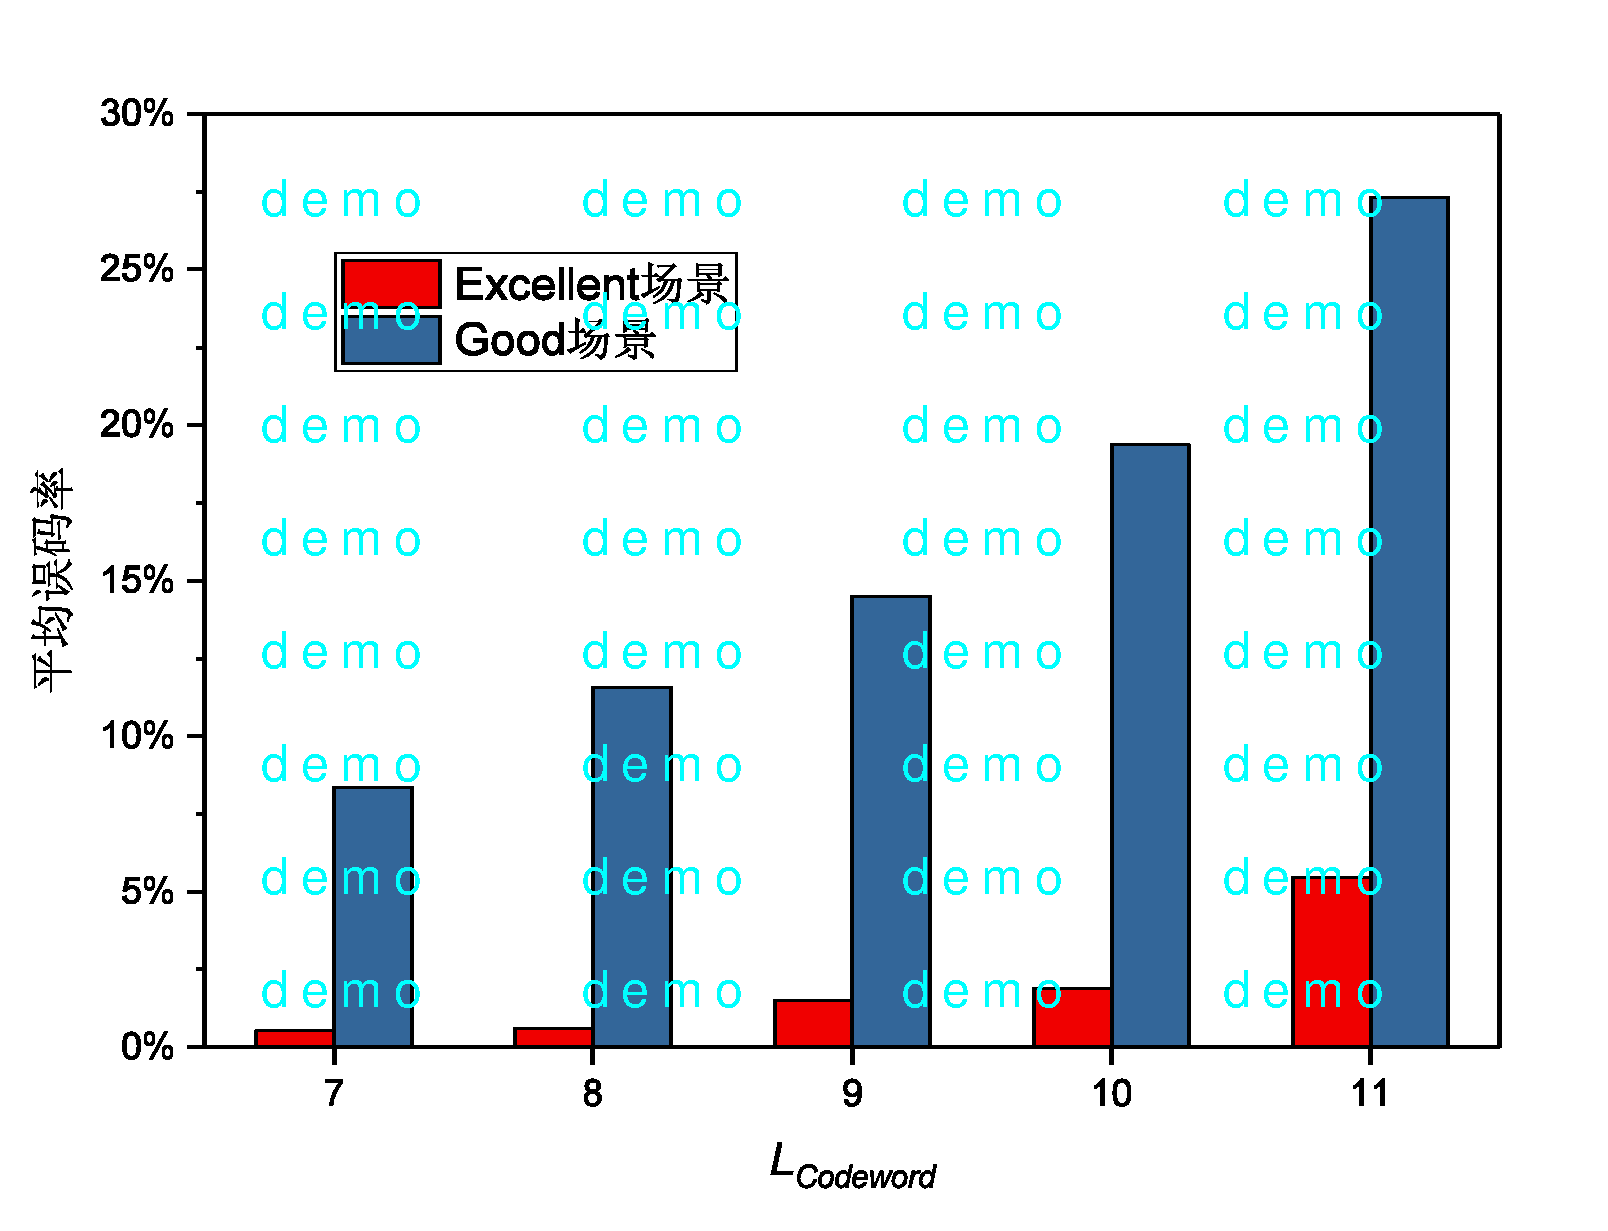
\includegraphics[width=0.48\textwidth]{chapters/chapter4/figures/ber-scenarios.pdf}
        }
        \subfigure[随机噪声场景]{
            \label{fig:4:results:ber:random}
            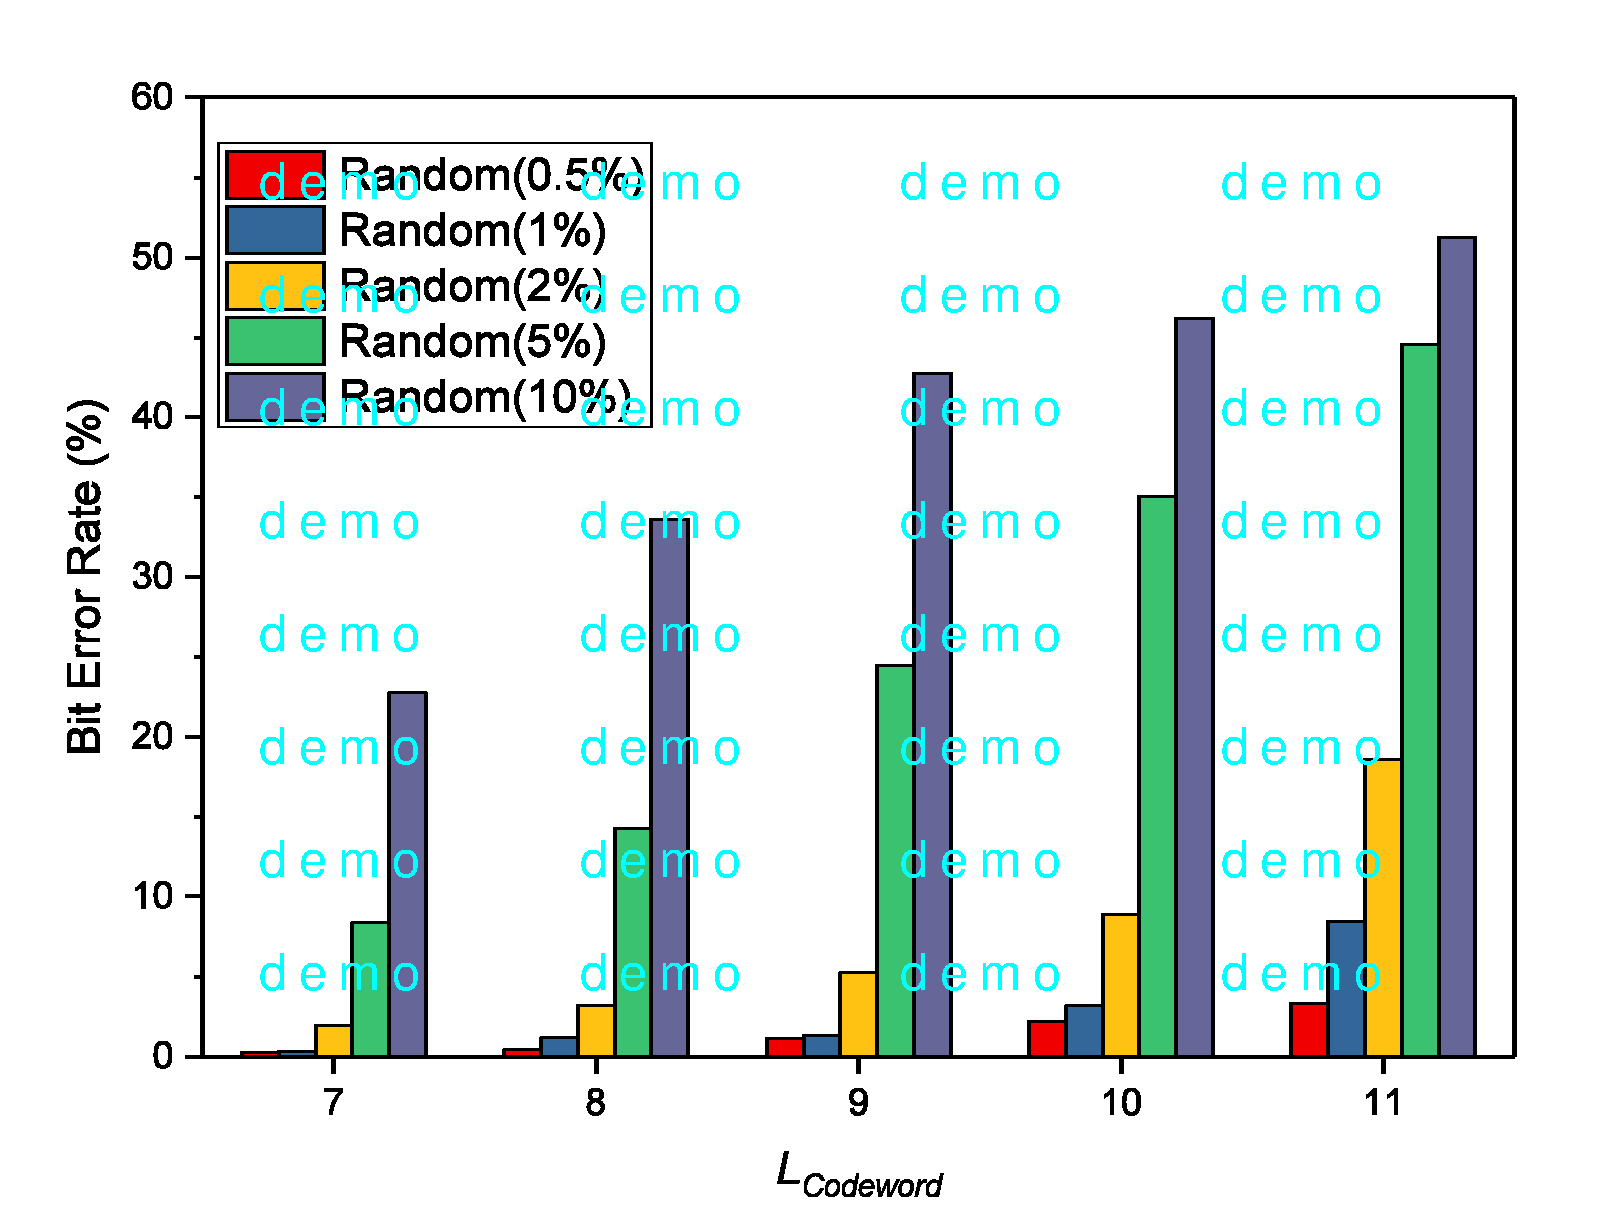
\includegraphics[width=0.48\textwidth]{chapters/chapter4/figures/ber-random.pdf}
        }
        \caption{时间隐通道的误码率水平}
        \label{fig:4:results:ber}
    \end{figure}
}

根据公式(\nref{equ:2:ber}),误码率也就是BER(Bit Error Rate)是评估鲁棒性的基本方式。各场景下的误码率水平如图\nref{fig:4:results:ber},其中图\nref{fig:4:results:ber:scenario}为Excellent及Good场景测试结果,图\nref{fig:4:results:ber:random}为随机噪声下的测试结果。

根据测试结果,随着$L_{Codeword}$的增长,误码率水平显著增加。由于$L_{Codeword}$ bits的数据需要$2^{L_{Codeword}}$个数据包完成调制,因此增大$L_{Codeword}$导致累积丢包数增加,码字鉴别准确率降低,时间隐通道的鲁棒性减弱,误码率升高。

网络噪声,尤其是随机丢包对该时间隐通道的影响显著。Excellent场景中的传输可靠性,明显优于Good场景。对比图\nref{fig:4:results:ber:random}中随机噪声下的误码率,Excellent场景与{$1\ \%$}随机噪声的结果相近,Good场景与{$10\ \%$}随机噪声的结果相近,与抓包场景下的丢包率基本一致(表\nref{tab:3:capture-results})。测试结果表明,随机丢包是对该时间隐通道的主要干扰。

在满足抗检测性要求,即$L_{Codeword}\ge 9$的基础上,该时间隐通道在Excellent场景下可以保证{$2\ \%$}左右的误码率;Good场景中误码率水平上升至{$15\ \%$}左右,对传输可靠性存在考验。因此,该时间隐通道构建方法,适用于网络状况较好的场景,高噪声场景中无法完全保证正确性。

\subsection{传输性能测试}
\label{chap:zigzag:results:throughput}

\insertTable{
	\begin{table}[htbp]
      \centering
      \caption{基于Zigzag映射矩阵时间隐通道的传输性能}
      \label{tab:4:results:throughput}
          \begin{tabular*}{0.8\textwidth}{@{\extracolsep{\fill}}cccccc}
            \toprule
            \multirow{2}{*}{指标} 
            & \multicolumn{5}{c}{$L_{Codeword}$} \\
            & 7 & 8 & 9 & 10 & 11 \\
            \midrule
            传输速率\ (bps) & 2.73 & 1.56 & 0.88 & 0.49 & 0.27 \\
            信道容量\ (bpp) & 0.027 & 0.016 & 0.009 & 0.005 & 0.003 \\
            \bottomrule
          \end{tabular*}
    \end{table}
}

根据公式(\nref{equ:4:throughput}),该时间隐通道的传输性能只与参数$L_{Codeword}$有关。不同参数下的传输性能如表\nref{tab:4:results:throughput},传输速率与$L_{Codeword}$呈负相关。在满足隐蔽性的前提下,当$L_{Codeword}=9$时,达到最高性能{0.88\ bps},增大$L_{Codeword}$导致性能按照$1/2$的比例依次衰减。

从传输性能的角度考虑,降低$L_{Codeword}$可以有效提升传输速率,但带来的代价是抗检测能力的衰退,违背了时间隐通道的前提。尤其是对基于主动丢包的时间隐通道来说,主动丢弃的数据包越多,用户通话质量受到的影响越大,同样影响隐蔽性。

\subsection{构建代价测试}
\label{chap:zigzag:results:cost}

\insertFigure{
	\begin{figure}[htbp]
        \centering
        \subfigure[Excellent场景的视频质量]{
            \label{fig:4:results:vq-excellent}
            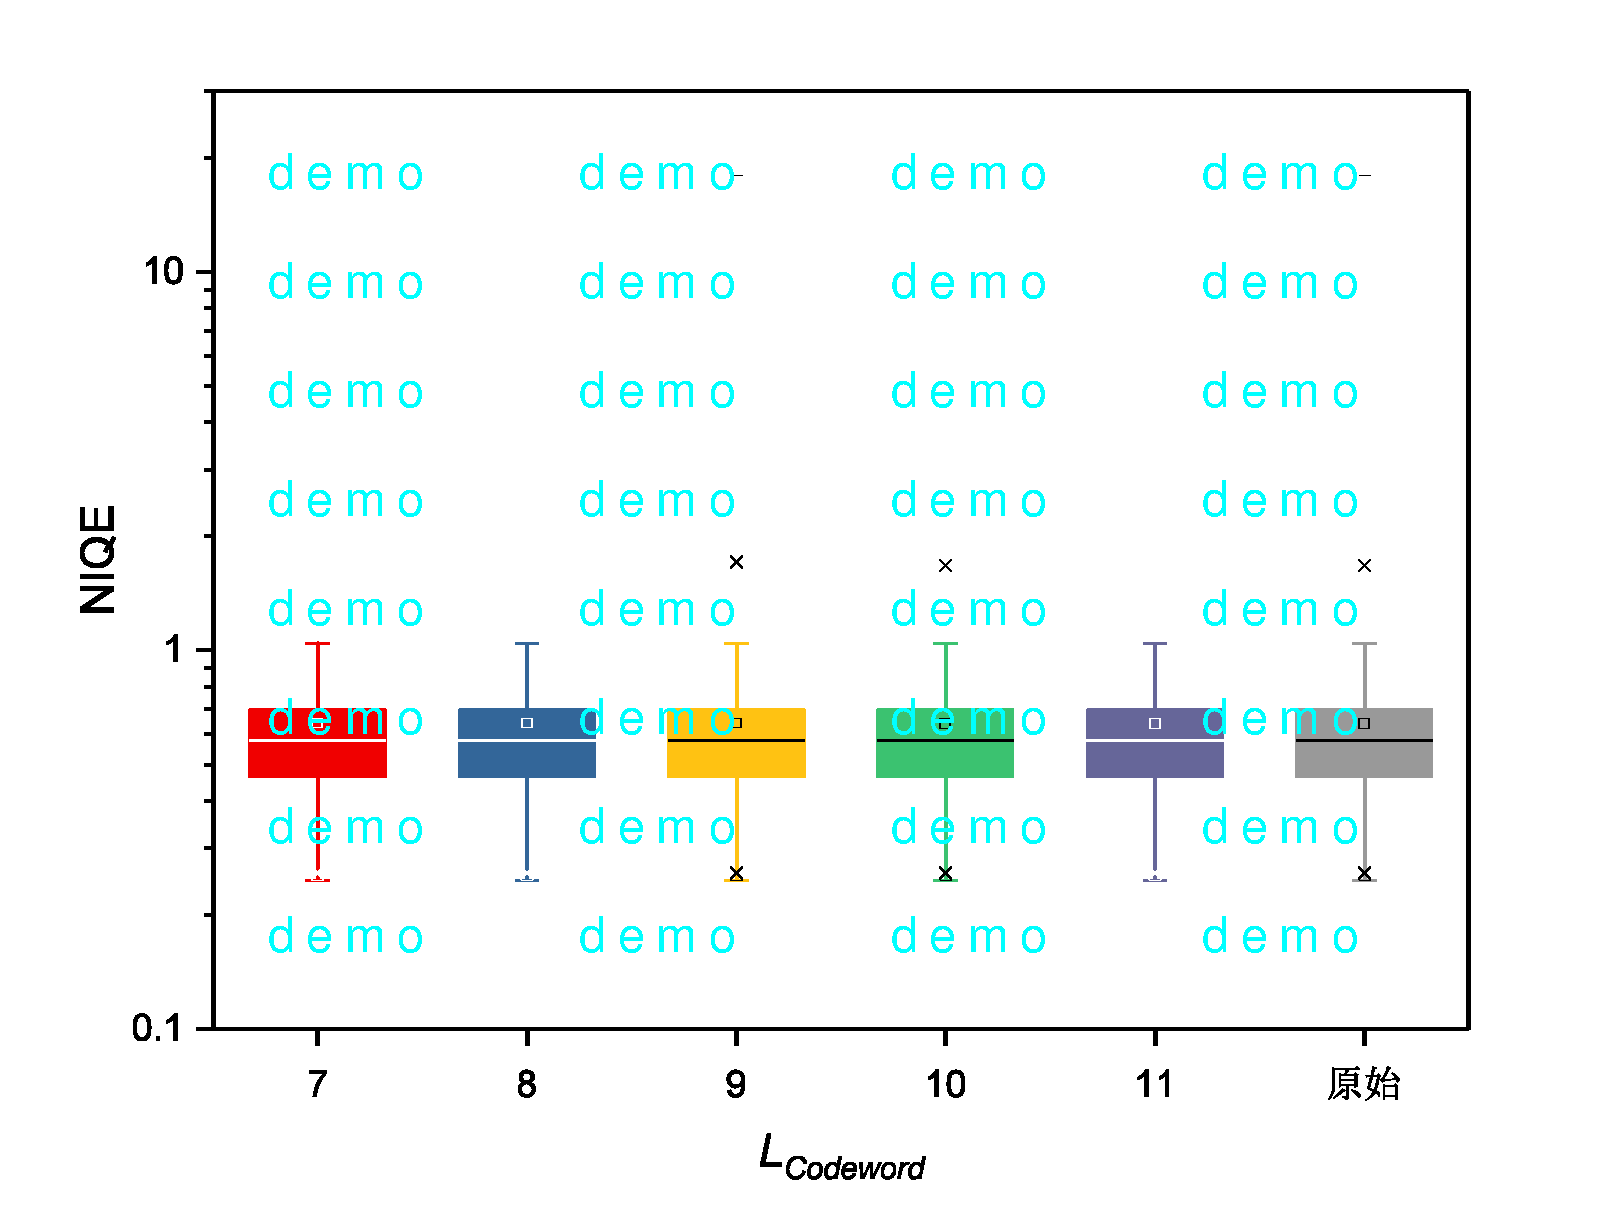
\includegraphics[width=0.48\textwidth]{chapters/chapter4/figures/vq-excellent.pdf}
        }
        \subfigure[Good场景的视频质量]{
            \label{fig:4:results:vq-good}
            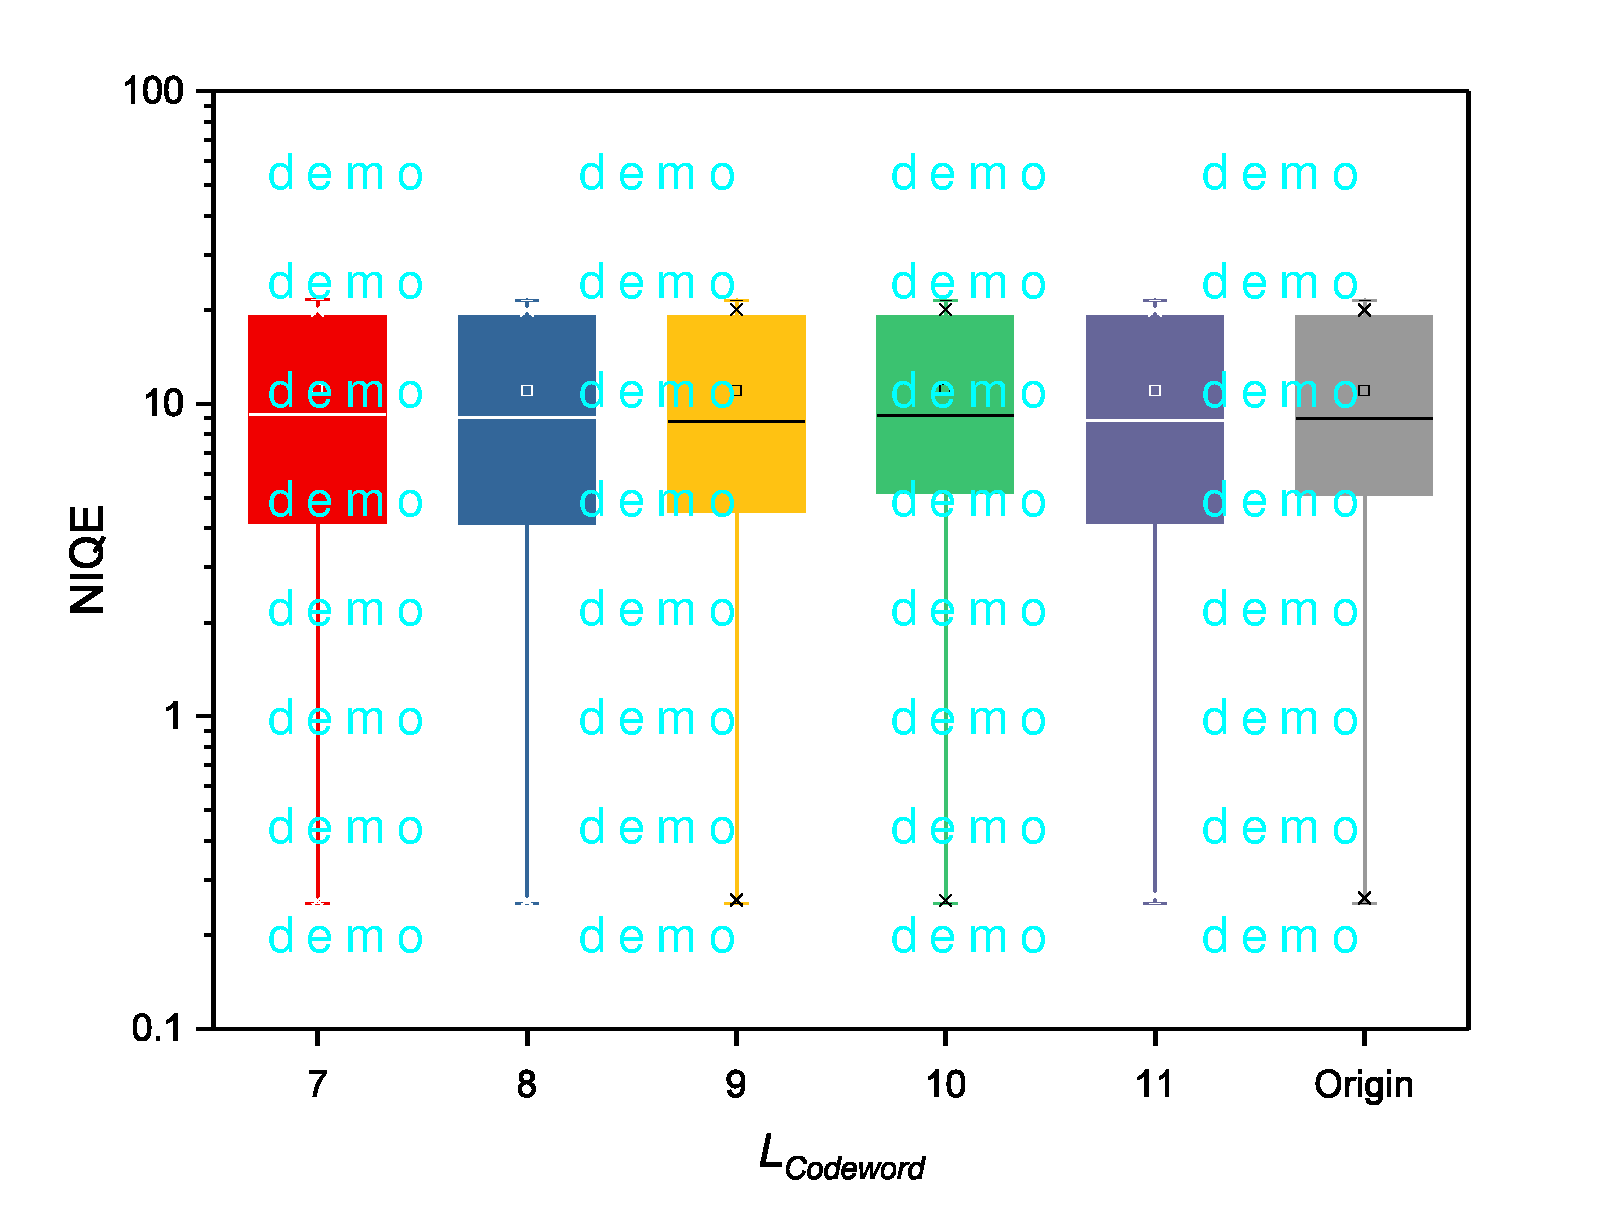
\includegraphics[width=0.48\textwidth]{chapters/chapter4/figures/vq-good.pdf}
        }
        \caption{时间隐通道的NIQE视频质量评估结果}
        \label{fig:4:results:vq}
    \end{figure}
}

基于Zigzag映射矩阵的时间隐通道,建立在VoLTE视频信道中,因此接收方的视频质量是评估构建代价的重要方面。根据表\nref{tab:4:parameters},当$L_{Codeword}\ge 9$时,构建时间隐通道导致的丢包率低于$0.2\%$,远小于网络噪声产生的丢包比例。

为评估视频质量,采用NIQE(Natural Image Quality Evaluator)无参照评价指标\nupcite{7094273},对视频中的所有帧进行质量评估,并判断视频整体的质量是否发生明显变化。\nupcite{7122356}NIQE反映了图像的失真程度,计算结果越大,证明图像质量越差。\nupcite{CoDLaCDAfMI,10.1145/3210424.3210434,6353522}视频质量评估结果如图\nref{fig:4:results:vq},Good场景下的NIQE值显著高于Excellent场景,证明Good场景中的通话体验受网络噪声干扰明显。

两种场景中,通过对比NIQE图像质量的范围和均值,证明时间隐通道没有产生显著质量损失。Excellent场景中,NIQE值多数在1以下,得益于较好的传输质量,时间隐通道产生的影响有限。Good场景中,原始的视频质量已经处于较差水平,虽然时间隐通道导致NIQE值发生了改变,但总体没有出现明显的差异。通过对比,该时间隐通道不会导致视频质量发生显著改变,满足时间隐通道低代价的要求。

\subsection{结论}
\label{chap:zigzag:results:conclusion}

\insertFigure{
	\begin{figure}[htbp]
        \centering
        \subfigure[Excellent场景下的综合评估]{
            \label{fig:4:results:sum:excellent}
            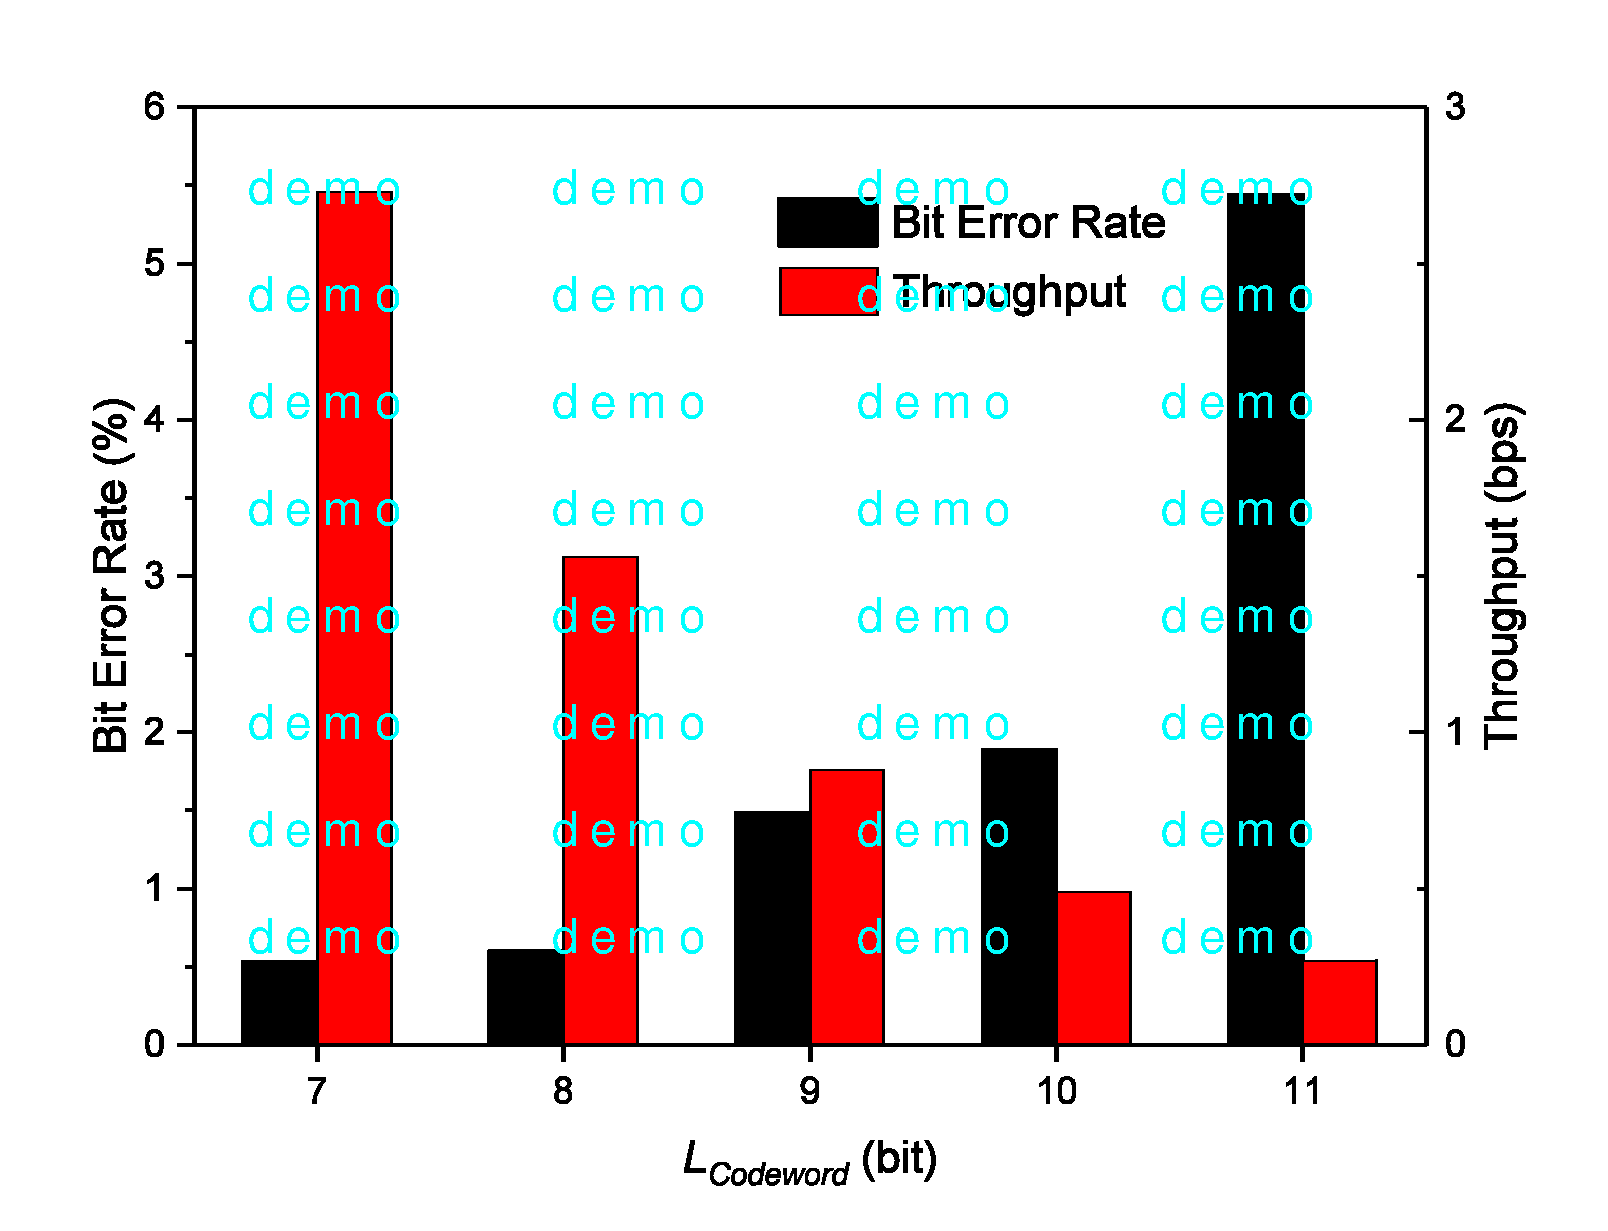
\includegraphics[width=0.48\textwidth]{chapters/chapter4/figures/sum-excellent.pdf}
        }
        \subfigure[Good场景下的综合评估]{
            \label{fig:4:results:sum:good}
            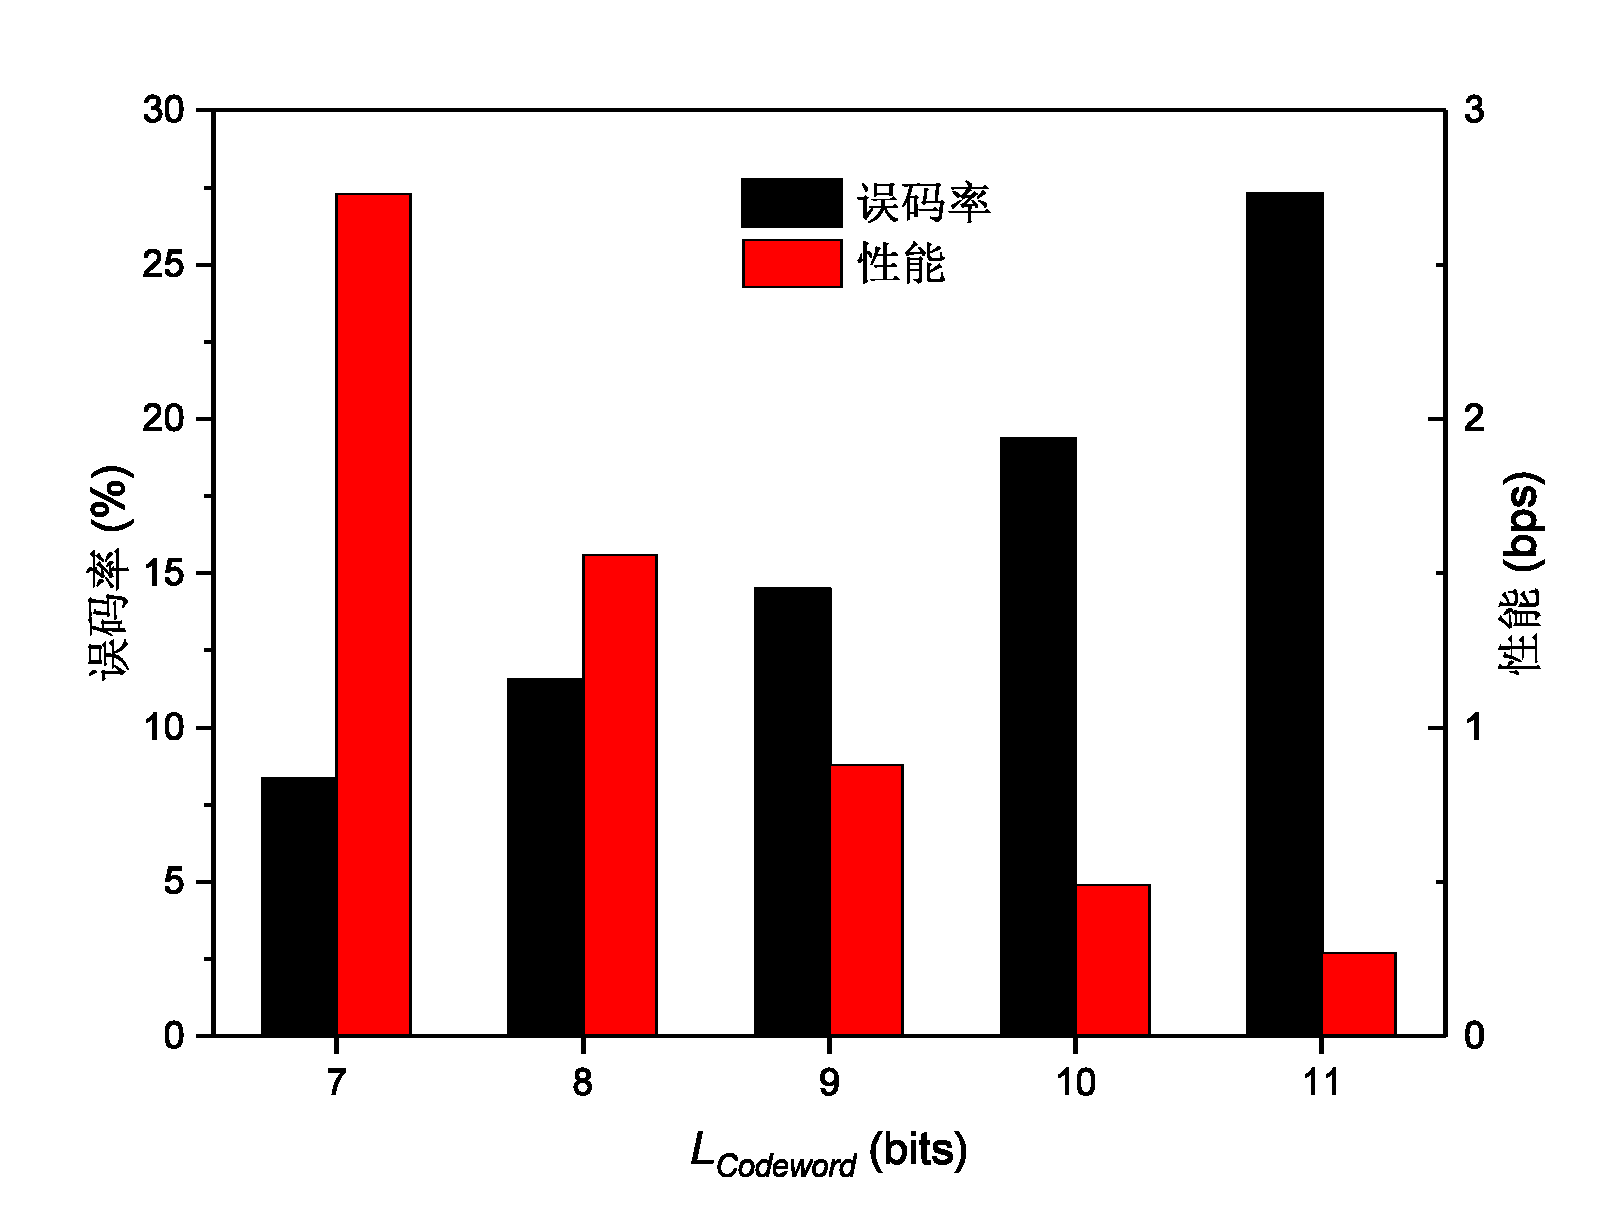
\includegraphics[width=0.48\textwidth]{chapters/chapter4/figures/sum-good.pdf}
        }
        \caption{基于Zigzag映射矩阵的时间隐通道综合评估}
        \label{fig:4:results:sum}
    \end{figure}
}

如图\nref{fig:4:results:sum},该时间隐通道的鲁棒性和传输性能均与$L_{Codeword}$呈负相关。结合本文\nref{chap:zigzag:results:undetectability}抗检测能力评估结果,该时间隐通道的最优$L_{Codeword}$为9,在该参数下能够通过所有的抗检测能力测试,并且具有{0.88\ bps}的传输性能及{0.5\ \%}的误码率。

\insertTable{
	\begin{table}[htbp]
      \centering
      \caption{基于Zigzag映射矩阵的时间隐通道横向比较}
      \label{tab:4:results:compare}
          \begin{tabular*}{0.85\textwidth}{@{\extracolsep{\fill}}cccc}
            \toprule
            时间隐通道构建方法 & 传输性能 & 信道容量 & 误码率 \\
            \midrule
            SCC\nupcite{10.1007/978-3-642-16435-4_15} & & 0.2$\sim$ 0.8 bpp & 2\% \\
            AFTC\nupcite{7347395} & & 0.5 bpp & 4\% \\
            CoCo\nupcite{10.1007/978-3-642-24178-9_22} & & 0.1$\sim$ 0.5 bpp & 4\% \\
            SPCC\nupcite{8288828} & 0.7$\sim$ 3 bps & & 0.9\% \\
            Zigzag-CTC & 0.88 bps & 0.009 bpp & 1.5\% \\
            \bottomrule
          \end{tabular*}
    \end{table}
}

表\nref{tab:4:results:compare}对比了几种时间隐通道的性能及误码率水平,分别为SCC\nupcite{10.1007/978-3-642-16435-4_15}、AFTC\nupcite{7347395}、CoCo\nupcite{10.1007/978-3-642-24178-9_22}、SPCC\nupcite{8288828}及本时间隐通道构建方法Zigzag-CTC。由于宿主信道的区别,时间隐通道的信道容量存在差异,但在传输性能方面,该时间隐通道可以达到时间隐通道的基本水平。在鲁棒性方面,该时间隐通道的最低误码率水平,与其它时间隐通道基本保持一致,达到了设计要求。